% Options for packages loaded elsewhere
\PassOptionsToPackage{unicode}{hyperref}
\PassOptionsToPackage{hyphens}{url}
%
\documentclass[
]{article}
\usepackage{lmodern}
\usepackage{amssymb,amsmath}
\usepackage{ifxetex,ifluatex}
\ifnum 0\ifxetex 1\fi\ifluatex 1\fi=0 % if pdftex
  \usepackage[T1]{fontenc}
  \usepackage[utf8]{inputenc}
  \usepackage{textcomp} % provide euro and other symbols
\else % if luatex or xetex
  \usepackage{unicode-math}
  \defaultfontfeatures{Scale=MatchLowercase}
  \defaultfontfeatures[\rmfamily]{Ligatures=TeX,Scale=1}
\fi
% Use upquote if available, for straight quotes in verbatim environments
\IfFileExists{upquote.sty}{\usepackage{upquote}}{}
\IfFileExists{microtype.sty}{% use microtype if available
  \usepackage[]{microtype}
  \UseMicrotypeSet[protrusion]{basicmath} % disable protrusion for tt fonts
}{}
\makeatletter
\@ifundefined{KOMAClassName}{% if non-KOMA class
  \IfFileExists{parskip.sty}{%
    \usepackage{parskip}
  }{% else
    \setlength{\parindent}{0pt}
    \setlength{\parskip}{6pt plus 2pt minus 1pt}}
}{% if KOMA class
  \KOMAoptions{parskip=half}}
\makeatother
\usepackage{xcolor}
\IfFileExists{xurl.sty}{\usepackage{xurl}}{} % add URL line breaks if available
\IfFileExists{bookmark.sty}{\usepackage{bookmark}}{\usepackage{hyperref}}
\hypersetup{
  pdftitle={Workshop 2\_Nonlinear Models},
  pdfauthor={Rachel Prokopius},
  hidelinks,
  pdfcreator={LaTeX via pandoc}}
\urlstyle{same} % disable monospaced font for URLs
\usepackage[margin=1in]{geometry}
\usepackage{graphicx,grffile}
\makeatletter
\def\maxwidth{\ifdim\Gin@nat@width>\linewidth\linewidth\else\Gin@nat@width\fi}
\def\maxheight{\ifdim\Gin@nat@height>\textheight\textheight\else\Gin@nat@height\fi}
\makeatother
% Scale images if necessary, so that they will not overflow the page
% margins by default, and it is still possible to overwrite the defaults
% using explicit options in \includegraphics[width, height, ...]{}
\setkeys{Gin}{width=\maxwidth,height=\maxheight,keepaspectratio}
% Set default figure placement to htbp
\makeatletter
\def\fps@figure{htbp}
\makeatother
\setlength{\emergencystretch}{3em} % prevent overfull lines
\providecommand{\tightlist}{%
  \setlength{\itemsep}{0pt}\setlength{\parskip}{0pt}}
\setcounter{secnumdepth}{-\maxdimen} % remove section numbering

\title{Workshop 2\_Nonlinear Models}
\author{Rachel Prokopius}
\date{1/23/2020}

\begin{document}
\maketitle

\hypertarget{objectives}{%
\section{Objectives}\label{objectives}}

The objective of the analysis was to fit light-response curves to data
collected at Harvard Forest in Massachusetts in order to better estimate
net ecosystem exchange (NEE) during periods of photosynthesis (day) and
plant respiration (night). These estimations will inform researchers
about the photosynthetic potential and ecosystem respiration for the
studied area of Harvard Forest.

\hypertarget{methods}{%
\section{Methods}\label{methods}}

\hypertarget{site-information-include-a-map-of-the-harvard-forest-site}{%
\subsection{Site Information (include a map of the harvard forest
site)}\label{site-information-include-a-map-of-the-harvard-forest-site}}

\begin{figure}
\centering
\includegraphics{C:/Users/Rachel Prokopius/Documents/FALCON HD/Graduate School/First Year/Spring Semester/Quantitative Ecology/Reproducible Science/Harvard Forest.jpg}
\caption{site image and map}
\end{figure}

Images from Google Maps and
\url{https://harvardforest.fas.harvard.edu/about-us}

Harvard Forest is a deciduous forest that is part of the sciences
program at Harvard College. The specific study site is found at the
following GPS coordinates:

Latitude: 42.53 Longitude: -72.19 Elevation: 330

The study site is a cool and moist temperature forest, with mean annual
temperatures ranging from -7°C to 20°C. Precipitation is fairly
consistent throughout the year.The dominant tree species found in the
area are Red oak (\emph{Quercus rubra}), Red maple (\emph{Acer rubrum}),
Black birch (\emph{Betula lenta}), White pine (\emph{Pinus strobus})and
Eastern hemlock (\emph{Tsuga canadensis}).

Data was collected from Environmental Measurement Station Eddy Flux
Towers (EMS) in the study area. The data set used in the analysis
includes hourly measurements of NEE in exchange per unit ground area,
air temperature in °C, and photosynthetically active radiation (PAR) in
nanometers. Measurements were attempted every hour by the EMS tower
beginning at 1 am on January 1st, 1991, and concluding at midnight on
January 1st, 2017.

\hypertarget{photosynthetic-potential}{%
\subsection{Photosynthetic Potential}\label{photosynthetic-potential}}

The equation used to estimate photosynthetic potential of the study site
was NEE \textasciitilde{} (a1 * PAR * ax)/(a1 * PAR + ax) + r, where a1,
ax and r are all parameters that need to be estimated for the model.

\hypertarget{estimate-initial-values-for-the-photosynthetic-potential-model-using-selfstart}{%
\subsubsection{Estimate initial values for the photosynthetic potential
model using
selfStart:}\label{estimate-initial-values-for-the-photosynthetic-potential-model-using-selfstart}}

load(``\textasciitilde/Desktop/NLM\_Workshop.RData'') library(nlstools)
lrcModel \textless- function(PAR, a1, ax, r) \{ NEE \textless- (a1 * PAR
* ax)/(a1 * PAR + ax) + r return(NEE) \}

lrc.int \textless- function (mCall, LHS, data)\{ x \textless-
data\(PAR y <- data\)NEE r \textless- max(na.omit(y), na.rm=T) ax
\textless- min(na.omit(y), na.rm=T) a1 \textless- (r + ax)/2

a1{[}a1 \textgreater{} 0{]}\textless- -0.1 r{[}r \textgreater{} 50{]}
\textless- ax*-1 r{[}r \textless{} 0{]} \textless- 1 value = list(a1,
ax, r) names(value) \textless- mCall{[}c(``a1'', ``ax'', ``r''){]}
return(value) \}

SS.lrc \textless- selfStart(model=lrcModel,initial= lrc.int)

iv \textless- getInitial(NEE \textasciitilde{} SS.lrc(`PAR', ``a1'',
``ax'', ``r''), data = day{[}which(day\$MONTH == 07),{]}) iv \#\#\#
Create a dataframe to store month parameter values a1, ax and r
(parms.Month):

parms.Month \textless- data.frame( MONTH=numeric(), a1=numeric(),
ax=numeric(), r=numeric(), a1.pvalue=numeric(), ax.pvalue=numeric(),
r.pvalue=numeric(), stringsAsFactors=FALSE, row.names=NULL)
parms.Month{[}1:12, 1{]} \textless- seq(1,12,1)

\hypertarget{write-a-function-to-fit-the-model-and-extract-paramter-values-a1-ax-and-r-nee.day}{%
\subsubsection{Write a function to fit the model and extract paramter
values a1, ax and r
(nee.day):}\label{write-a-function-to-fit-the-model-and-extract-paramter-values-a1-ax-and-r-nee.day}}

nee.day \textless- function(dataframe)\{ y = nls( NEE \textasciitilde{}
(a1 * PAR * ax)/(a1 * PAR + ax) + r, dataframe, start=list(a1=
iv\(a1 , ax= iv\)ax, r= iv\$r), na.action=na.exclude, trace=F,
control=nls.control(warnOnly=T))

y.df \textless- as.data.frame(cbind(t(coef(summary(y)) {[}1:3, 1{]}),
t(coef(summary(y)) {[}1:3, 4{]}))) names(y.df)
\textless-c(``a1'',``ax'', ``r'', ``a1.pvalue'', ``ax.pvalue'',
``r.pvalue'') return (y.df )\}

\hypertarget{write-a-loop-to-fit-monthly-curves-and-add-paramters-to-a-dataframe-parms.month}{%
\subsubsection{Write a loop to fit monthly curves and add paramters to a
dataframe
(parms.Month):}\label{write-a-loop-to-fit-monthly-curves-and-add-paramters-to-a-dataframe-parms.month}}

try(for(j in unique(day\$MONTH))\{

iv \textless- getInitial(NEE \textasciitilde{} SS.lrc(`PAR', ``a1'',
``ax'', ``r''), data = day{[}which(day\$MONTH == j),{]})

y3 \textless- try(nee.day(day{[}which(day\$MONTH == j),{]}), silent=T)

try(parms.Month{[}c(parms.Month\$MONTH == j ), 2:7 {]} \textless-
cbind(y3), silent=T) rm(y3) \}, silent=T) parms.Month

\hypertarget{bootstrapping}{%
\subsubsection{Bootstrapping}\label{bootstrapping}}

boot.NEE \textless- data.frame(parms.Month{[}, c(``MONTH''){]}); names
(boot.NEE) \textless- ``MONTH''
boot.NEE\(a1.est <- 0 boot.NEE\)ax.est\textless- 0
boot.NEE\(r.est<- 0 boot.NEE\)a1.se\textless- 0
boot.NEE\(ax.se<- 0 boot.NEE\)r.se\textless- 0

for( j in unique(boot.NEE\$Month))\{

y1 \textless-day{[}which(day\$MONTH == j),{]}

iv \textless- getInitial(NEE \textasciitilde{} SS.lrc(`PAR', ``a1'',
``ax'', ``r''), data = y1)

day.fit \textless- nls( NEE \textasciitilde{} (a1 * PAR * ax)/(a1 * PAR
+ ax) + r, data=y1, start=list(a1= iv\(a1 , ax= iv\)ax, r= iv\$r),
na.action=na.exclude, trace=F, control=nls.control(warnOnly=T))

try(results \textless- nlsBoot(day.fit, niter=100 ), silent=T) try(a
\textless-
t(results\(estiboot)[1, 1:3], silent=T) try(names(a) <- c('a1.est', 'ax.est', 'r.est'), silent=T) try( b <- t(results\)estiboot){[}2,
1:3{]}, silent=T) try(names(b) \textless- c(`a1.se', `ax.se', `r.se'),
silent=T) try(c \textless- t(data.frame(c(a,b))), silent=T)

try(boot.NEE{[}c(boot.NEE\$MONTH == j), 2:7{]} \textless- c{[}1, 1:6{]},
silent=T) try(rm(day.fit, a, b, c, results, y1), silent=T) \}

lrc \textless- merge( parms.Month, boot.NEE, by.x=``MONTH'',
by.y=``MONTH'') lrc

\hypertarget{ecosystem-respiration}{%
\subsection{Ecosystem Respiration}\label{ecosystem-respiration}}

\hypertarget{estimate-initial-values-for-the-photosynthetic-potential-model-using-selfstart-1}{%
\subsubsection{Estimate initial values for the photosynthetic potential
model using
selfStart:}\label{estimate-initial-values-for-the-photosynthetic-potential-model-using-selfstart-1}}

load(``\textasciitilde/Desktop/NLM\_Workshop.RData'') library(nlstools)
trcModel \textless- function(TA, a, b) \{ y=a * exp(b*TA) return(y) \}

trc.int \textless- function (mCall, LHS, data)\{ x \textless-
data\(TA  y <- data\)NEE

a \textless-1.00703982 + -0.08089044* (min(na.omit(y))) b \textless-
0.051654 + 0.001400 * (min(na.omit(y)))

value = list(a, b) names(value) \textless- mCall{[}c(``a'', ``b''){]}
return(value) \}

SS.trc \textless- selfStart(model=trcModel,initial= trc.int)

\hypertarget{create-a-dataframe-to-store-month-parameter-values-a1-ax-and-r-parms.month.night}{%
\subsubsection{Create a dataframe to store month parameter values a1, ax
and r
(parms.Month.night):}\label{create-a-dataframe-to-store-month-parameter-values-a1-ax-and-r-parms.month.night}}

parms.Month.night \textless- data.frame(

MONTH=numeric(),

a=numeric(),

b=numeric(),

a.pvalue=numeric(),

b.pvalue=numeric(), stringsAsFactors=FALSE, row.names=NULL)

parms.Month.night {[}1:12, 1{]} \textless- seq(1,12,1)

\hypertarget{write-a-function-to-fit-the-model-and-extract-paramter-values-a1-ax-and-r-nee.night}{%
\subsubsection{Write a function to fit the model and extract paramter
values a1, ax and r
(nee.night):}\label{write-a-function-to-fit-the-model-and-extract-paramter-values-a1-ax-and-r-nee.night}}

nee.night \textless- function(dataframe)\{y.df = nls(NEE
\textasciitilde{} a * exp(b*TA),

\begin{verbatim}
                                        dataframe, start=list(a= iv$a ,b=iv$b),
                                        
                                        na.action=na.exclude, trace=F,
                                        
                                        control=nls.control(warnOnly=T))
\end{verbatim}

y.df \textless- as.data.frame(cbind(t(coef(summary(y.df)){[}1:2, 1{]}),
t(coef(summary(y.df)) {[}1:2, 4{]})))

names(y.df) \textless- c(``a'', ``b'', ``a.pvalue'', ``b.pvalue'')

return(y.df)\}

\hypertarget{write-a-loop-to-fit-monthly-curves-and-add-paramters-to-a-dataframe-parms.month.night}{%
\subsubsection{Write a loop to fit monthly curves and add paramters to a
dataframe
(parms.Month.night):}\label{write-a-loop-to-fit-monthly-curves-and-add-paramters-to-a-dataframe-parms.month.night}}

try(for(j in unique(night\$MONTH))\{

iv \textless- getInitial(NEE \textasciitilde{} SS.trc(`TA', ``a'',
``b''), data = night{[}which(night\$MONTH == j),{]})

y4 \textless- try(nee.night(night{[}which(night\$MONTH == j),{]}),
silent=T)

try(parms.Month.night{[}c(parms.Month.night\$MONTH == j ), 2:5 {]}
\textless- cbind(y4), silent=T) rm(y4) \}, silent=T)

parms.Month.night

\hypertarget{bootstrapping-1}{%
\subsubsection{Bootstrapping}\label{bootstrapping-1}}

boot.NEE.night \textless- data.frame(parms.Month.night{[},
c(``MONTH''){]}); names (boot.NEE.night) \textless- ``MONTH''
boot.NEE.night\(a.est <- 0 boot.NEE.night\)b.est \textless- 0
boot.NEE.night\(a.se <- 0 boot.NEE.night\)b.se \textless- 0

for ( j in unique(boot.NEE.night\$MONTH))\{

y5 \textless-night{[}which(night\$MONTH == j),{]}

iv \textless- getInitial(NEE \textasciitilde{} SS.trc(`TA', ``a'',
``b''), data = y5)

night.fit \textless- nls( NEE \textasciitilde{} (a * exp(b * TA)),
data=y5, start=list(a= iv\(a , b= iv\)b), na.action=na.exclude, trace=F,
control=nls.control(warnOnly=T))

try(results \textless- nlsBoot(night.fit, niter=100 ), silent=T) try(a
\textless-
t(results\(estiboot)[1, 1:2], silent=T)  try(names(a) <- c('a.est','b.est'), silent=T)  try(b <- t(results\)estiboot){[}2,
1:2{]}, silent=T) try(names(b) \textless- c(`a.se',`b.se'), silent=T)
try(c \textless- t(data.frame(c(a,b))), silent=T)

try(boot.NEE.night{[}c(boot.NEE.night\$MONTH == j), 2:5{]} \textless-
c{[}1, 1:4{]}, silent=T) try(rm(night.fit, a, b, c, results, y1),
silent=T) \} trc \textless- merge( parms.Month.night,
boot.NEE.night,by.x=``MONTH'', by.y=``MONTH'') \# Merge dataframes trc

\hypertarget{results}{%
\section{Results}\label{results}}

\begin{figure}
\centering
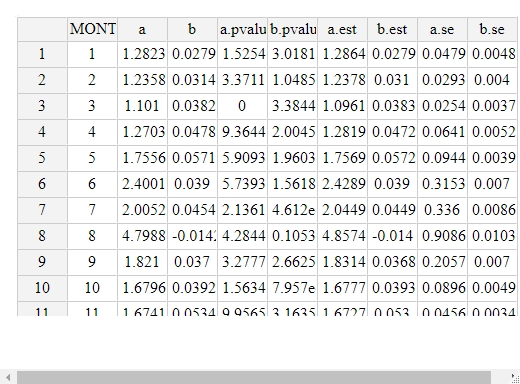
\includegraphics{C:/Users/Rachel Prokopius/Documents/FALCON HD/GitHub/Reproducible-science/respiration.jpeg}
\caption{respiration}
\end{figure}

\begin{figure}
\centering
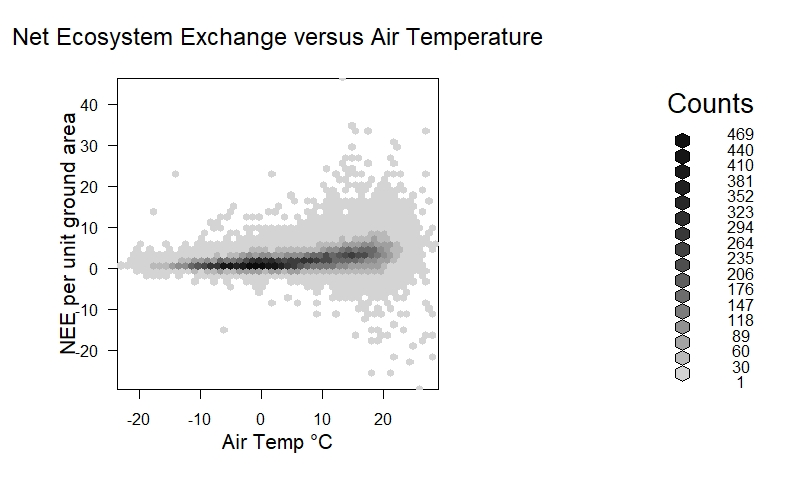
\includegraphics{C:/Users/Rachel Prokopius/Documents/FALCON HD/GitHub/Reproducible-Science/Rplot02.jpeg}
\caption{graph}
\end{figure}

\hypertarget{discussion-1-paragrapgh}{%
\section{Discussion (1 paragrapgh)}\label{discussion-1-paragrapgh}}

\end{document}
